\section{Minimalism}
\scriptsize{Features} {\tiny core part of minimalist syntax, refers to a feature value not a feature label, e.g. verbs might have the features past, plural, etc.
}\\
\scriptsize{categorial features} {\tiny POS, phrase symbol, e.g. A, N, V, NP, VP...
}\\
\scriptsize{$\phi$-features} {\tiny features relevant for agreement, e.g. PERSON, NUMBER, GENDER
}\\
\scriptsize{case features} {\tiny e.g. nominative, accusative}\\
\scriptsize{strong features} {\tiny features may be strong or weak, strong features make syntactic objects move to higher positions
}\\
\scriptsize{interpretable/uninterpretable features} 
{\tiny interpretable in English\\
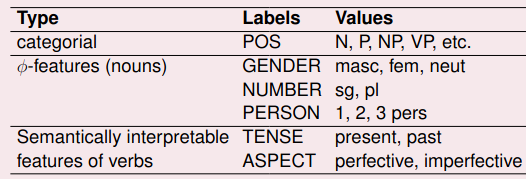
\includegraphics[scale=0.2]{interpretable.png}\\
uninterpretable in English\\
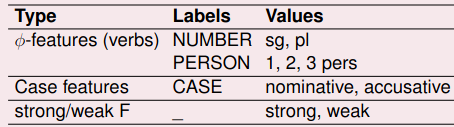
\includegraphics[scale=0.2]{uninterpretable.png}\\
differs corss-linguistically, e.g. GENDER feature is interpretable for English, not for German
}\\
\scriptsize{Feature Checking} 
{\tiny a core mechanism within Minimalist Syntax, links features with phrase structure, hence replaces traditional phrase structure rules\\
requirement: uninterpretable features must be checked, and once checked they delete\\
checking of categorial features: NP, NP with adjective, DP, VP\\
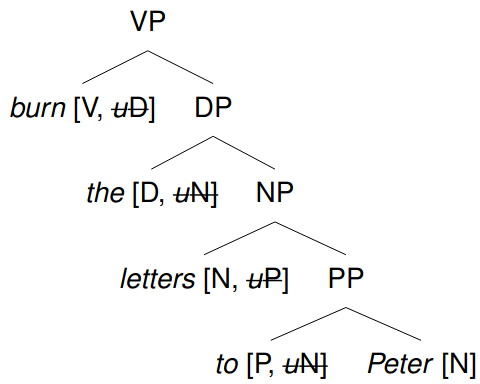
\includegraphics[scale=0.15]{feature-checking.png}\\
checking agreement features: Agree mechanism to check other features in addition to selectional features\\
agreement features can be checked in a sister node or further down the tree, whereas categorial features have to be checked in the sister node (or right below the sister node) of the feature to be checked\\
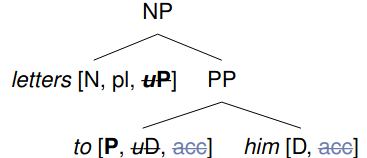
\includegraphics[scale=0.2]{agreement-features.png}
}\\
\scriptsize{Merge and Move} 
{\tiny
external merge (aka Merge): simply combines 2 elements like "the" and "book"\\
internal merge (aka Move($\alpha$): movement of constituents, adjoins some part of one linguistic object to the left of the respective object, the original position (i.e. trace) is indicated by <$\alpha$>\\
these have to be motivated by feature checking and essentially replaces phrase structure rules
}\\
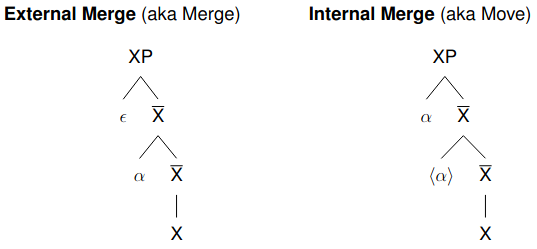
\includegraphics[scale=0.2]{merge.png}\\
\scriptsize{Phrase Structure} \\
{\tiny First merge - complements: combines a head with a single complement to create a complete phrase (XP)\\
Second merge - specifiers: combines a head with a specifier\\
little v: modelling ditransitives with reflexive pronouns, another higher level of the verb phrase, preferred by many practitioners of MP\\
Tense Phrase (TP): corresponds to IP in GB analysis\\
Complementizer Phrase (CP): in contrast to GB, full sentences in MP are always complementizer phrases; if C is empty, it still contributes to clause-type feature, e.g. Decl for declarative; the highest level phrase in MP\\
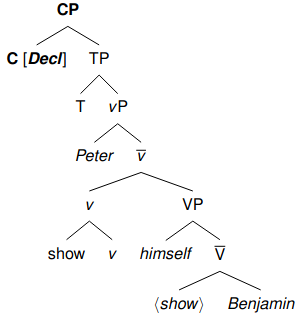
\includegraphics[scale=0.2]{cp.png}
}\\
\scriptsize{Differences between Minimalism and GB}
{\tiny structure building relies on feature checking not rewrite rules; there is just merge(external) and move(internal merge) applied in any order rather than D- and S- structure; case assignment no longer handled with the principle of government but by feature checking (Agree)}\\
\scriptsize{Pros}
{\tiny reduce the operations assumed for structure building (feature checking, merge and move) and hence more evolutionary plausible; 1 complement (first merge) and several specifiers (second merge) leads to a strictly binary structure without lots of unary branches (in X-bar theory)
}\\
\scriptsize{Cons}
{\tiny not fully formalized, hard to implement computationally; quickly fragmented into many divergent frameworks, development of implementations of large grammar fragments is hard
}